\section{Qualitätssicherung (Testprotokoll)} \label{Tests}

 	\subsection{Erläuterung der Userteststudie}
Um die Qualität zu gewährleisten, haben wir uns ein Studienkonzept überlegt. Dabei stellen wir unseren Probanden verschiedene Aufgaben in unserer App. Während sie die Aufgaben erfüllen, beobachten wir sie und bewerten ihre Leistungen mit vier möglichen Ausprägungen: 'sehr gut', 'gut', 'ok' und 'schlecht'. Wenn bei einer Aufgabe mehrheitlich mit 'ok' oder 'schlecht' bewertet wird, können wir daraus Verbesserungspotenzial ableiten.
Aus zeitlichen Gründen ist es uns nicht möglich eine größer angelegte Studie durchzuführen. Unsere Probanden beschränken sich auf Verwandte und Bekannte. Optimaler wäre eine größere und diversere Anzahl an Probanden ohne persönlichen Bezug.
Der Test beginnt für jeden User auf der Loginseite (Siehe Abschnitt \ref{Login}).
	
	\subsection{Useraufgaben und Bewertungen}
	
	\subsubsection{Registrieren Sie sich.}
	Verwenden Sie:
	\begin{itemize}
		\item E-Mail: [vorname]@mail.de
		\item Passwort: 123456 
	\end{itemize}
	\ \\
	\begin{tabular}{|>{$\rhd$ }lrl|}
		\hline
		sehr gut  & \mybar{2}\\
		gut  & \mybar{4}\\
		ok               & \mybar{0}\\
		schlecht         & \mybar{0}\\
		\hline
	\end{tabular}
	
	\paragraph{Kommentar:}\ \\
	Zwei Probanden mit der Bewertung \textbf{gut} haben zunächst Anmelden mit Registrieren verwechselt.
Ein Proband mit der Bewertung \textbf{gut} hatte Probleme den 'Sign up'-Knopf zu finden.

	
	\subsubsection{Melden Sie sich mit Ihren Nutzerdaten an.}
	\begin{tabular}{|>{$\rhd$ }lrl|}
		\hline
		sehr gut  & \mybar{6}\\
		gut  & \mybar{0}\\
		ok               & \mybar{0}\\
		schlecht         & \mybar{0}\\
		\hline
	\end{tabular}
	
	\paragraph{Kommentar:}\ \\
	Passiert nach der Registrierung automatisch.
	
	\subsubsection{Erstellen Sie eine Reise.}
	\begin{tabular}{|>{$\rhd$ }lrl|}
		\hline
		sehr gut  & \mybar{4}\\
		gut  & \mybar{2}\\
		ok               & \mybar{0}\\
		schlecht         & \mybar{0}\\
		\hline
	\end{tabular}
		
	\paragraph{Kommentar:}\ \\
	Ein Proband mit der Bewertung \textbf{sehr gut} empfand den 'currently involved'-Reiter auf der Reiseerstellenseite als verwirrend.
	
	\subsubsection{Öffnen Sie die Einladungsseite ihrer Reise.}
	\begin{tabular}{|>{$\rhd$ }lrl|}
		\hline
		sehr gut  & \mybar{5}\\
		gut  & \mybar{0}\\
		ok               & \mybar{1}\\
		schlecht         & \mybar{0}\\
		\hline
	\end{tabular}
			
	\paragraph{Kommentar:}\ \\
	Ein Proband mit der Bewertung \textbf{ok} lieferte keinen Kommentar. Dies ist in dem Sinne hervorzuheben, dass die Einladungsseite automatisch nach Erstellen der Reise aufgerufen wird.

	\subsubsection{Versuchen Sie einer Reise beizutreten, wenn Ihnen folgendes Bild geschickt wurde: (sieh Abb. \ref{fig:user_test_invite}).}
	
	\begin{figure}[H]
		\centering
		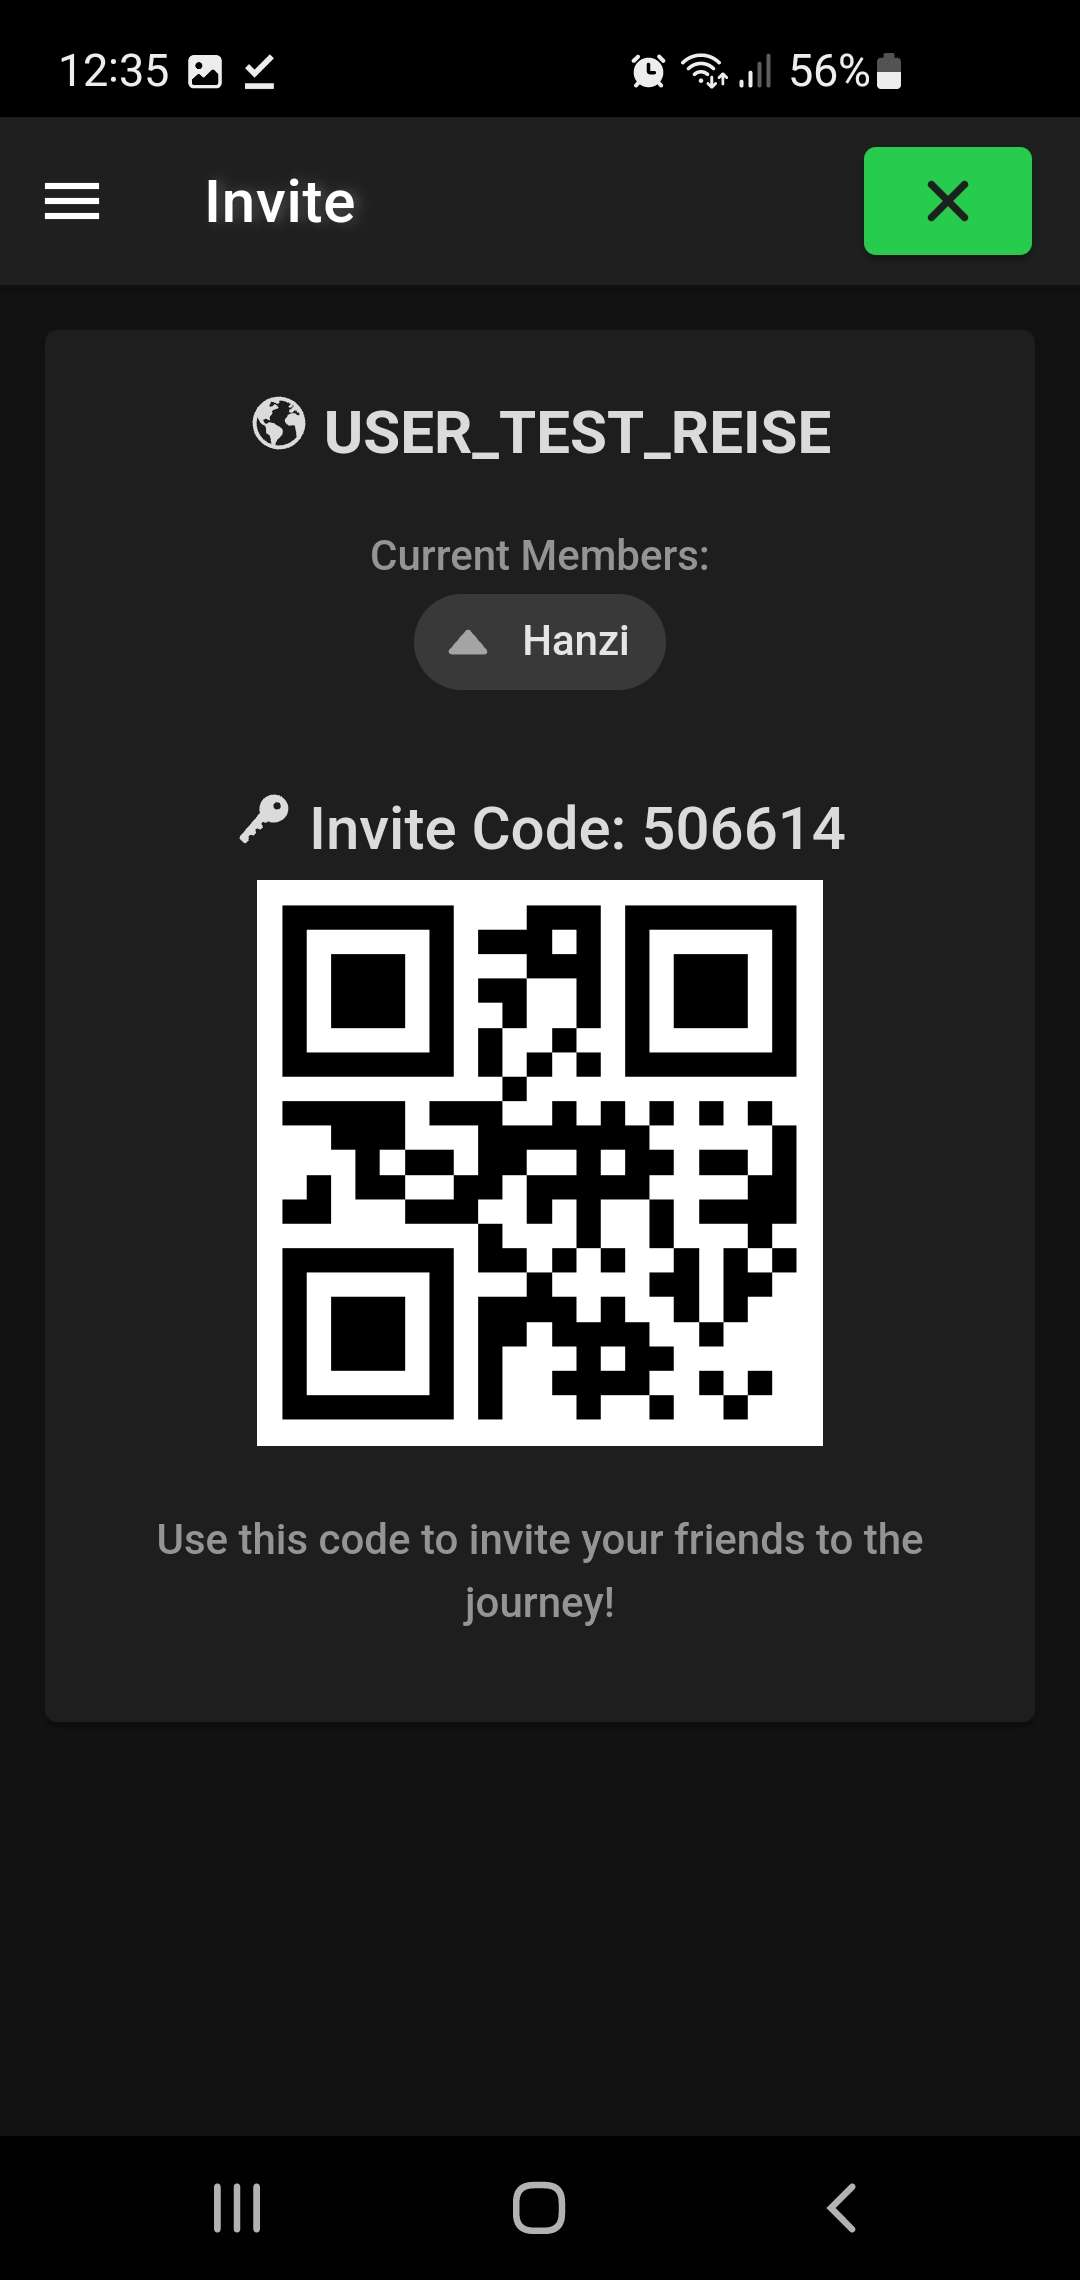
\includegraphics[width=0.3
		\textwidth]{img/user_test_invite}
		\caption[Usertest Einladung]{Usertesteinladung}
		%\captionsource{}
		\label{fig:user_test_invite}
	\end{figure}
	
	\begin{tabular}{|>{$\rhd$ }lrl|}
		\hline
		sehr gut  & \mybar{4}\\
		gut  & \mybar{0}\\
		ok               & \mybar{1}\\
		schlecht         & \mybar{1}\\
		\hline
	\end{tabular}
			
	\paragraph{Kommentar:}\ \\
	Ein Proband mit der Bewertung \textbf{sehr gut} empfand die Anweisung als verwirrend. Ein Proband
mit Bewertung \textbf{ok} bemängelt eine fehlende deutsche Übersetzung. 

\newpage

	\subsubsection{Erstellen Sie in der Reise 'User\_Test\_Reise' eine Ausgabe, bei der Sie 50 € für ein Mittagessen mit Hanz und Marie gezahlt haben.}
	\begin{tabular}{|>{$\rhd$ }lrl|}
		\hline
		sehr gut  & \mybar{2}\\
		gut  & \mybar{2}\\
		ok               & \mybar{2}\\
		schlecht         & \mybar{0}\\
		\hline
	\end{tabular}
			
	\paragraph{Kommentar:}\ \\
	Ein Proband mit der Bewertung \textbf{ok}:
	\begin{itemize}
		\item hätte Kategorie und Ausgabenbeteiligte fast übersprungen
		\item hat die Aufgabe zunächst missverstanden und sich nicht als Ausgabenbeteiligter eingetragen.
		\item wollte Teilnehmer mit in den Titel eingeben.
	\end{itemize}
	Ein Proband mit der Bewertung \textbf{ok} hat den Titel vergessen.


	\subsubsection{Bearbeite Sie die Zahlung zu 85 €.}
	\begin{tabular}{|>{$\rhd$ }lrl|}
		\hline
		sehr gut  & \mybar{5}\\
		gut  & \mybar{0}\\
		ok               & \mybar{1}\\
		schlecht         & \mybar{0}\\
		\hline
	\end{tabular}
			
				
	\paragraph{Kommentar:}\ \\
	-

	\subsubsection{Lassen Sie sich die Schulden der Reise anzeigen.}
	\begin{tabular}{|>{$\rhd$ }lrl|}
		\hline
		sehr gut  & \mybar{4}\\
		gut  & \mybar{2}\\
		ok               & \mybar{0}\\
		schlecht         & \mybar{0}\\
		\hline
	\end{tabular}
	
	\paragraph{Kommentar:}\ \\
	Ein Proband mit der Bewertung \textbf{gut} hatte zunächst innerhalb einer Ausgabe gesucht, dann aber die Seite
gefunden. Ein Proband mit der Bewertung \textbf{gut} hat Zahlungen und Schulden verwechselt.

	\subsubsection{Vermerken Sie, dass Marie 5 € zurückgezahlt hat.}
	\begin{tabular}{|>{$\rhd$ }lrl|}
		\hline
		sehr gut  & \mybar{2}\\
		gut  & \mybar{2}\\
		ok               & \mybar{2}\\
		schlecht         & \mybar{0}\\
		\hline
	\end{tabular}
			
	\paragraph{Kommentar:}\ \\
	Zwei Probanden mit den Bewertungen \textbf{gut} und \textbf{ok} empfanden es als verwirrend, dass bei Festhalten einer
Zahlung bereits der Betrag der Gesamtschulden eingetragen ist.

	\subsubsection{Erstellen Sie in der Reise 'User\_Test\_Reise' eine Ausgabe bei der Hanz für Sie beide ein Taxi am 03.01.23 für 100 € gezahlt hat.}
	\begin{tabular}{|>{$\rhd$ }lrl|}
		\hline
		sehr gut  & \mybar{5}\\
		gut  & \mybar{0}\\
		ok               & \mybar{1}\\
		schlecht         & \mybar{0}\\
		\hline
	\end{tabular}
			
	\paragraph{Kommentar:}\ \\
	Ein Proband mit der Bewertung \textbf{ok} hat Beteiligte und Titel vergessen.

	\subsubsection{Lassen Sie sich die Schulden der Reise erneut anzeigen. Ändern Sie die Währung zu £.}
	\begin{tabular}{|>{$\rhd$ }lrl|}
		\hline
		sehr gut  & \mybar{6}\\
		gut  & \mybar{0}\\
		ok               & \mybar{0}\\
		schlecht         & \mybar{0}\\
		\hline
	\end{tabular}
			
	\paragraph{Kommentar:}\ \\
	-
	
	\subsubsection{Halten Sie fest, dass Sie Marie die Schulden zurückgezahlt haben.}
	\begin{tabular}{|>{$\rhd$ }lrl|}
		\hline
		sehr gut  & \mybar{5}\\
		gut  & \mybar{0}\\
		ok               & \mybar{0}\\
		schlecht         & \mybar{1}\\
		\hline
	\end{tabular}
			
	\paragraph{Kommentar:}\ \\
	Auf der Umfrageseite stand zeitweise Hanz anstelle von Marie, dieser besitzt aber zu diesem
Zeitpunkt keine Schulden.


	\subsubsection{Ändern Sie die Sortierung für die Ausgaben der Reise 'User\_Test\_Reise'.}
	\begin{tabular}{|>{$\rhd$ }lrl|}
		\hline
		sehr gut  & \mybar{5}\\
		gut  & \mybar{1}\\
		ok               & \mybar{0}\\
		schlecht         & \mybar{0}\\
		\hline
	\end{tabular}
			
	\paragraph{Kommentar:}\ \\
	Es wurde ein Bug festgestellt. Reise sowie Reiseliste aktualisieren sich nicht. Ausgaben werden
nicht eingefügt, sondern sind erst nach erneutem Laden der Seite da. 
	
	\subsubsection{Löschen Sie alle Ausgaben der Reise 'User\_Test\_Reise'.}
	\begin{tabular}{|>{$\rhd$ }lrl|}
		\hline
		sehr gut  & \mybar{6}\\
		gut  & \mybar{0}\\
		ok               & \mybar{0}\\
		schlecht         & \mybar{0}\\
		\hline
	\end{tabular}
			
	\paragraph{Kommentar:}\ \\
	-
	
	\subsubsection{Archivieren Sie die von Ihnen erstellte Reise.}\label{Archivieren Sie die von Ihnen erstellte Reise.}
	\begin{tabular}{|>{$\rhd$ }lrl|}
		\hline
		sehr gut  & \mybar{0}\\
		gut  & \mybar{4}\\
		ok               & \mybar{0}\\
		schlecht         & \mybar{2}\\
		\hline
	\end{tabular}
			
	\paragraph{Kommentar:}\ \\
	Zwei Probanden mit der Bewertung \textbf{schlecht} haben den Button nicht gefunden und hatten auch
keine Idee wo er sein könnte.
	
	\subsubsection{Loggen Sie sich aus der App aus.}
	\begin{tabular}{|>{$\rhd$ }lrl|}
		\hline
		sehr gut  & \mybar{5}\\
		gut  & \mybar{1}\\
		ok               & \mybar{0}\\
		schlecht         & \mybar{0}\\
		\hline
	\end{tabular}
			
	\paragraph{Kommentar:}\ \\
	-
	
\subsection{Fazit der Userteststudie}
Wir sind mit dem Ergebnis der Userteststudie zufrieden. Die Probanden sind für erstmaliges Nutzen der App gut zurechtgekommen. Aus dem Ergebnis von Anweisung \ref{Archivieren Sie die von Ihnen erstellte Reise.} leiten wir
Verbesserdungsbedarf ab, zum Beispiel das Verwenden eindeutigerer Icons. Für den Archivieren-Button hatten wir
zeitweise ein passenderes Icon, allerdings bietet Ionic kein passendes Icon für die Umkehrfunktion (Entarchivieren), weshalb wir auf das Schloss-Icon zurückgreifen mussten.
Ein größeres Problem war die fehlende Validierung von Nutzereingaben. Diese Aufgabe war einem Gruppenmitglied zugeteilt worden, welches die Gruppe kurz vor Abgabe verlassen hat. Eine Erkenntnis für uns ist daher dafür zu sorgen solch eine essentielle Funktionalität rechtzeitig einem anderen Gruppenmitglied zuzuweisen, damit diese noch implementiert werden kann.
Außerdem haben wir anhand der Rückmeldungen der Probanden gelernt die Anweisungen der Nutzerstudie noch präziser zu formulieren.
